\chapter{Chemotherapy}
\label{chap:chemo}

As the number of cancer treatments increases, together with the dose ranges that will be explored starting earlier in the clinical trial process as encouraged by the \ac{FDA} in Project Optimus, so does the need for more computationally guided approach to dose selection. While it is not experimentally feasible to explore the full spectrum of possible drug doses and regimens, especially if these parameters are allowed to vary from one drug injection to the next, a mathematical framework such as the one presented here can be used to sort through the countless possible combinations. In this work, we build upon a mathematical model that quantitatively captures the complex interactions between tumor, immune system, and a chemotherapy drug. The proposed model is calibrated with experimental data of \ac{SCID} mice implanted with aggressive treatment-resistant glioma tumors and treated with cyclopsphamide under a variety of dosing regimens to capture impact of drug dose and schedule on both the tumor and the immune cells. Next, by applying a numerical implementation of optimal control to this model, we show that the \ac{MDOR} for this mouse model is neither metronomic nor \ac{MTD} but instead constitutes administering a lower dose in the beginning of treatment, and then a larger dose after 35 days, resulting in maximal tumor control for the first 60 days. The discovered regimen can be interpreted from the lens of "press-pulse" notion in species extinction theory, when most frequent and expansive mass species extinctions occurred when ``press" disturbances on the population (such as climate or sea level change) weakened and destabilized populations over many generations, and were then followed by a ``pulse" disturbance that cause extensive mortality. This work highlights the ability of well constructed and validated mathematical models to provide insights into improved dosing and scheduling for long term tumor reduction, which can then be evaluated experimentally. By expanding application of optimal control to other mouse models and beyond, we can begin to uncover optimal treatment strategies in a quantitatively-guided way.

\section{Background}
Finding the appropriate dosing and scheduling of a chemotherapy drug for a given tumor type is an exceedingly challenging task. The current standard of care limits the regimens used primarily to daily dose and \ac{MTD} treatments. A \ac{MTD} regimen attempts to reduce the tumor burden as much as tolerable by the patient with each treatment. In addition to potential severe side effects, the treatment can lose efficacy rapidly and give rise to drug resistance \cite{zahreddine2013mechanisms,kareva2015metronomic,shah2016limiting}. In addition to simply selectively killing non-resistant cells in a ``Darwin''-like fashion, high levels of cytotoxicity caused by \ac{MTD} treatments can greatly weaken the host immune system \cite{kareva2015metronomic}, removing an important line of defense against resistant cells. Metronomic or ``intermittent'' chemotherapy treatments with lower dose amount and higher frequency than \ac{MTD} were shown to be able to induce an immune response alongside the cytotoxicity of the drug towards cancerous cells, at least in mouse models, and under specific treatment conditions \cite{kepp2009immunogenic,kepp2011molecular,doloff2012vegf,kroemer2013immunogenic,vacchelli2014trial,bracci2014immune,wu2014metronomic,chen2014intermittent,bezu2015combinatorial,wu2015metronomic,wu2016metronomic}. Furthermore, if the treatments are given too regularly such as seen in the case of daily dose treatments, the elicited immune response can be greatly attenuated \cite{wu2014metronomic}. An optimal treatment should ideally strike the right balance of both eliciting a strong immune response and still providing enough cytotoxicity towards cancer cells from the chemotherapy drug \cite{park2019goldilocks,tran2020delicate}.

Only a subset of chemotherapy drug are known to induce this immunogenic cancer cell death pathway that produces a strong anti-cancer immune response. This effect is dependent on various factors that include the tumor type or subtype, the regimen that is being applied, as well as the class of chemotherapy drug. Drugs that are able to induce this immunostimulatory effect include cyclophopshamide, anthracyclines, 5-fluorouracil, mitoxantrone, idarubicin, and doxorubicin \cite{zitvogul2008,chen2013chemoimmunotherapy,bracci2014immune,vacchelli2014trial,pol2015trial}. In addition to using the appropriate drug, eliciting an anti-tumor immune response requires an appropriate balance of drug dosing and scheduling \cite{wu2018immunogenic,park2019goldilocks,tran2020delicate}. There remains much to be understood about the complex dynamics that leads to the observation of a strong immune recruitment in a 6-day repeating schedule (Q6D) at 140 mg/kg per dose of cyclophosphamide administered to treat GL261 glioma and 9L gliosarcoma tumors, a response that a daily dose or maximum tolerated treatment dose does not elicit to a noticeable extent \cite{wu2014metronomic,chen2014intermittent,doloff2012vegf}. Understanding how treatment strategies affect the dynamics and interactions between the drug, the immune system, and the tumor holds the key to developing more effective treatment strategies.

Developing realistic mathematical models of these biological interactions is a challenging task due to the number of phenomena that need to be considered. The immune system alone needs various considerations for immune cell types, chemicals (cytokines and chemokines), and various roles that these immune cells can play (e.g. T-cells can be cytoxotic or memory). Each of these immune components has distinct dynamics that makes it difficult to predict the aggregate behavior of the biological system as a whole from its various components. There are additional factors to consider such as individual variability between patients, variability in the tumor, the drug used for treatment, and how the chosen drug is administered. The fact that a cytototoxic drug like cyclophosphamide can be both immunostimulatory and immunosuppressive in a metronomic treatment makes designing accurate mathematical representations of the interactions at play particularly difficult. There is a rich literature on mathematical models that attempt to capture the mechanisms behind cancer chemotherapy and how it affects the immune system \cite{de2005clinical,de2006mixed,ciccolini2017pharmacokinetics,park2019goldilocks}. There are also considerations that have been made to model drug resistance \cite{greene2019mathematical}.

A central idea that guided this chapter was coming up with a realistic representation of the phenomena that arise during a metronomic chemotherapy: drug-mediated suppression of the immune system, recruitment of immunostimulatory factors by the immunogenic cancer cell death pathway, drug resistance that arises during treatment, tumor-immune interactions, tumor growth, and drug pharmacokinetics. The parameters of the developed mathematical model are fitted to a large dataset of tumor trajectories for which the treatment conditions were varied \cite{wu2014metronomic}. Using this mathematical representation of the drug-immune-tumor interactions, a numerical optimal control scheme was used to find a potentially better treatment schedule for the analyzed data. The results illustrate the potential of model-guided chemotherapy treatments can potentially be one day used in the clinic.

\section{Modeling}

A major challenge of modeling the immune system resides in the complex interactions between its components. Even using the \ac{SCID} mouse model as was used in  \cite{wu2014metronomic}, which eliminates the impact of B and T cells, maintains the impact of innate immune cells, such as NK cells, macrophages, dendritic cells, and neutrophils. An attempt to model each of these immune components individually greatly increases  model complexity and the number of parameters to be fitted, and may come even at a detriment to the model's ultimate utility. Instead, experimentally observed immune data from \cite{wu2014metronomic} can be clustered into the following three categories by response type :
\begin{itemize}
	\item an early response from immunostimulatory chemokines (e.g. CXCL9, CXCL10, CXCL11)
	\item a correlated response from immune cell markers shortly after the release of immunostimulatory chemokines
	\item the response of vascular endothelial growth factor A (VEGF-A), which is inversely correlated with the other measured immune cell markers
\end{itemize}

To build upon the previous modeling effort for this data set \cite{tran2020delicate}, and use it to apply optimal control techniques to find potential dosing and scheduling regimes that might be superior to the ones that were tested in the following section. 
The model takes into account the effects of immune recruitment, drug resistance, and the complex interactions between the drug, the tumor, and the immune system. Compared to the model introduced in \cite{tran2020delicate}, here it has been modified to become more generalizable; specific modifications and the corresponding rationale are given below.
\begin{subequations} \label{eq:chemo1}
	\begin{align} 
		\dot{T}(t) &=  k_{a} T(t) - \frac{k_{b}C(t)T(t)}{k_{c}C(t)+T(t)} - k_{d}T(t)I(t),\\
		\dot{I}(t) &= q X(t) -k_{e}T(t)I(t)-k_{f}C(t)I(t)-k_{g}Y(t)I(t)-k_{h}I,\\
		\dot{X}(t) &= \frac{q C(t)T(t)}{k_{i}C(t)+T(t)}-k_{j}X(t)-k_{k}X(t)Y(t),\\
		\dot{Y}(t) &= \frac{I(t)}{k_l+I(t)} - k_{m}Y(t) C(t),\\
		\dot{C}{t} &= u(t) - \frac{k_1 C(t)}{k_2 + C(t)}.
	\end{align}
\end{subequations}
subjected to the following initial conditions $[T,I,X,Y,C](0)=[T_0,\frac{k_n}{k_o+T_0},0,0,0]$. The unit of phenomenological variables $C$, $I$, $X$, and $Y$ is 1, and the unit of variable $T$, tumor volume, is mm$^3$. A detailed description for each parameter and variable used in this model is presented in Table~\ref{table:chemo1}.
%
\begin{landscape}
\begin{table}
	\centering
	\caption{Definition of the variables and parameters used in the model~\eqref{eq:chemo1}.}
	\begin{tabular}{c c c c}
		\hline
		Parameter/Variable   & Unit          & Value & Definition\\ \hline
		$T(t)$       & mm$^3$         & $T(0)=T_0$& Tumor volume\\ 
		$I(t)$       & 1         & $I(0)=\frac{k_n}{k_o+T_0}$& Immune system \\ 
		$X(t)$       & 1         & $X(0)=0$ & Immunostimulatory intermediate\\ 
		$Y(t)$       & 1         & $Y(0)=0$ & Immunosuppressor intermediate\\ 
		$C(t)$       & 1         & $C(0)=0$ & Drug (input)\\ 
		$k_a$       & 1/day         & $1.555\times 10^{-1}$ & Tumor growth rate\\ 
		$k_b$       & mm$^3$/day    & $1.334\times 10^{-1}$ & Cytotoxic effect rate of the drug on the tumor\\ 
		$k_c$       & mm$^3$        & $5.195\times 10^{-1}$ & Saturation term of drug and tumor interaction \\
		$k_d$       & 1/day         & $1.992\times 10^{-2}$ & Cytotoxic effect of the immune system on the tumor \\ 
		$k_e$       & 1/day/mm$^3$  & $3.463\times 10^{-5}$ & Negative effect of the tumor on the immune system \\ 
		$k_f$       & 1/day         & $2.940\times 10^{-1}$ & Cytotoxic effect of the drug on the immune system\\ 
		$k_g$       & 1/day     & $6.497\times 10^{-1}$ & The immunosuppressor effect on the immune system\\ 
		$k_h$       & 1/day     & $1.369\times 10^{-1}$ & The immune system natural decay rate\\ 
		$k_i$       & mm$^3$    & $1.837\times 10^{-1}$ & Saturation term of the immunostimulatory recriutment term caused by the tumor debris\\ 
		$k_j$       & 1/day     & $5.987\times 10^{-4}$ & The immunostimulatory natural decay rate \\ 
		$k_k$       & 1/day     & $1.249\times 10^{-1}$ & The immunosuppression effect rate \\
		$k_l$       & 1         & $1.435\times10^{-3}$  & Saturation term of immunosuppressor increase in response to the immune system  \\ 
		$k_m$       & 1/day     & $3.997\times10^{-5}$  & Cytotoxic effect of the drug on the immunosuppressor intermediate\\
		$k_n$       & mm$^3$    & $1.966\times 10^{+3}$ & Initial immune system parameter \\ 
		$k_o$       & mm$^3$    & $2.040\times10^{-4}$  & Initial immune system parameter \\ 
		$k_1$       & 1/day     & $1.525\times 10^{+2}$ & Mechaelis-Menton elimination term parameter\\ 
		$k_2$       & 1         & $5.594\times 10^{+3}$ & Mechaelis-Menton elimination term parameter\\ 
		$q$       & 1 /day        & 1 & Makes the phenamenological variables unitless. \\ 
		\hline
	\end{tabular}
	\label{table:chemo1}
\end{table}
\end{landscape}
%
Tumor growth inhibition data has been previously used to identify the parameters in our previous work \cite{tran2020delicate}. Here, the objective function is defined to compare the tumor and immune data for fitting the parameters in model~\eqref{eq:chemo1}. It is made up of two components: $f_1(x)$ the error with respect to the tumor data and $f_2(x)$ the error with respect to the immune data. Where $x$ is a vector of fitting parameters represented in the model and introduced in table \ref{table:chemo1}, and $X$ is the physically meaningful parameters space search defined by upper bound and lower bound of each parameter. This is to incorporate both the experimentally measured tumor growth inhibition and immune markers into the model.
%
\begin{equation} \label{objective}
	\min_{x\in X}\; \qquad w_1\times\underbrace{f_1(x)}_\textrm{based on the measured tumor volume}\;\;+\; w_2\times\underbrace{f_2(x)}_\textrm{based on the average of measured immune system markers}.
\end{equation}
%
A best set of parameters represented in table \ref{table:chemo1} are identified to result in minimum value of the objective function. To remove bias of the fitted parameters to immune or tumor data, the weights $w_1$ and $w_2$ are selected such that both error terms of similar magnitude. In this work, the values for $w_1$ and $w_2$ were picked to be 1 and 18, respectively.

For calculating the objective function the simulated tumor data and immune data are needed to be compared with the experimentally measured data. Comparing the experimental tumor data to its corresponding simulated data is obvious because they constitute similar measurements. 
In the case of the immune data, there are 18 measured correlated immune markers excluding the immunostimulatory chemokines and VEGF-A. Since there is only one variable \textit{I} accounting for the drug-induced immune response, these relative gene expression values were averaged. 

Another challenge for calculating the mean immune data in the objective function is that the experimental data was normalized as a ratio of the measured gene expression in the untreated case at a specific day. Thus, before the values are to be compared, the values of $I$ from the simulated model needs to be averaged between the different starting volumes, then normalized with respect to the simulated untreated case.

The error function used for the immune system is given by:
\begin{equation}
	f_2(x) = \frac{|I_{simulated}-I_{measured}|}{I_{measured}+\epsilon}
\end{equation}
with $\epsilon$ representing a small deviation. Where $I_{simulated}$ is the immune system level $[I(t_1), I(t_2), \dots, I(t_n)]$ at the same time points that $I_{measured}$ the immune system markers were measured $t_1, t_2, \dots, t_n$, and  $f_2(x)$ is the sum of the errors for all of the experimental immune data points.

\section{Optimization}

In the previous section we used the model to evaluate the relationship between drug exposure and mean tumor volume. The model revealed that more frequent dosing would counter-intuitively require higher drug exposure to achieve lower final tumor volume, while less frequent drug administration may achieve good tumor reduction with lower \ac{AUC}, unlike is expected from \ac{MTD} protocol. In this section we apply optimal control to further explore additional drug administration strategies, which may go beyond administering a fixed dose at fixed time intervals. 

The optimal drug dosing strategy based on the mathematical model and fitted parameters defined in the previous section is implemented using a numerical optimal control software GPOPS-II~\cite{patterson2014gpops}. The output is shown in  Fig.~\ref{fig:oc}. To set up the optimal control problem, the following objective function and boundary conditions are used: 

\begin{align}  \label{eq:ocp}
	\begin{split}
		\min_{u(t)} & \quad T(t_f), \\
		s.t. & \quad 
		\begin{bmatrix}
			0 \\ 0 \\ 0 \\ 0 \\ 0 \\ 0
		\end{bmatrix} 
		\leq
		\begin{bmatrix}
			C(t) \\ T(t) \\ I(t) \\ X(t) \\ Y(t) \\ u(t)
		\end{bmatrix}
		\leq
		\begin{bmatrix}
			C_m \\ T_m \\ I_m \\ X_m \\ Y_m \\ u_m
		\end{bmatrix},
		\\
		& \quad \int_0^{t_f} u(t) dt \leq U_m.
	\end{split}
\end{align}
%
where $C_m=780$ mg/kg, $T_m=4000$ mm$^3$, $I_m=100$, $X_m=1000$, and $Y_m=1000$ are the maximum acceptable values for the state variables. Input upper bound $u_m$ is set to $1000$ 1/day (SI Figs.\ref{fig:OP1} and \ref{fig:OP2}) and $60$ 1/day (SI Figs. \ref{fig:OP3} and \ref{fig:OP4}) to setup two different optimal control problems for the numerical solver. Different input bounds are helpful to understand how instant large dose of drug is making different in the optimal control results. Boundary conditions for the state variables were identified through metronomic treatment simulations based on treatment constraints that were deemed reasonable. $U_m$ is the maximum possible total amount of drug used in aggregate. Other constraints were placed, such as $C_m$ to limit the maximum value of the phenomenological drug variable. The objective function $T(t_f)$ minimizes the tumor volume at the final time $t_f=60$ of the treatment. The boundary conditions $C_m=780$, and $U_m=1400$ are based on the standard 140 mg/kg Q6D treatment. Fig.~\ref{fig:oc}(a) compares the treatment outcome and administered drug dose of metronomic treatment with the optimal control problem with input bound of $u_m=60$.
%
%\begin{figure}[H]
%	\centering
%	\begin{subfigure}[b]{\textwidth}
%		\centering
%		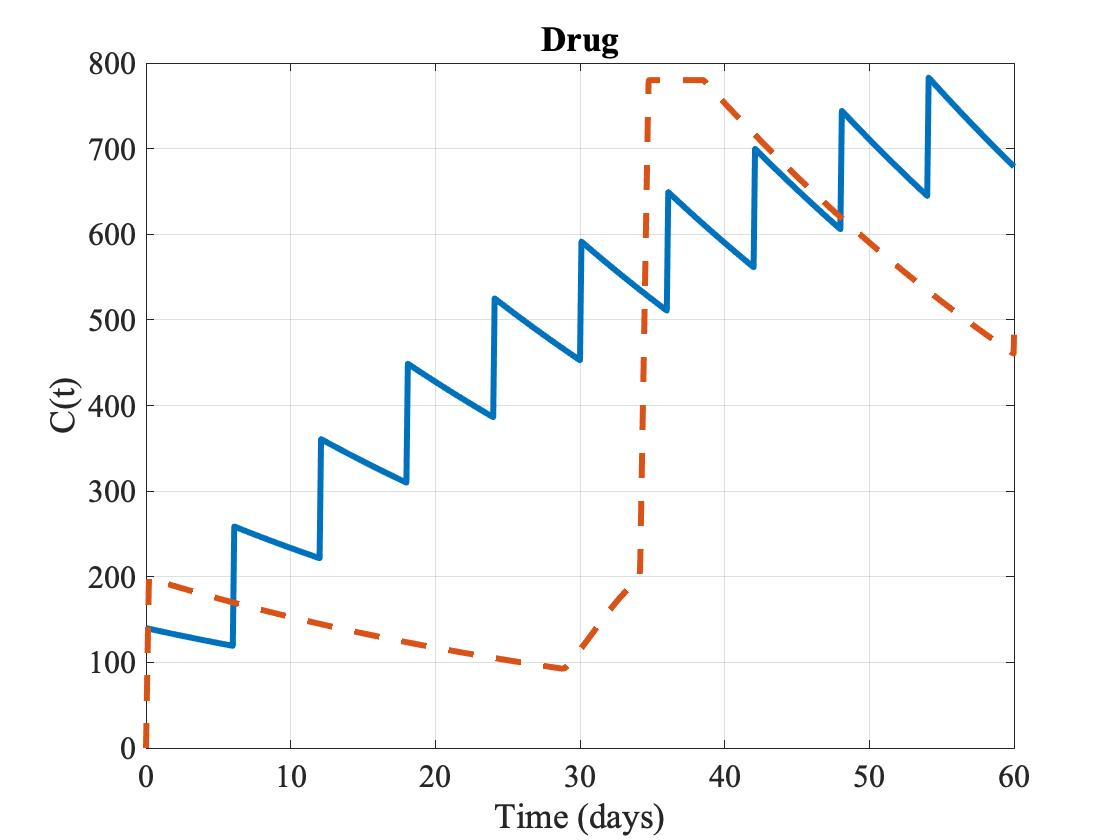
\includegraphics[width=0.49\textwidth]{fig/chemo_1.jpeg}
%		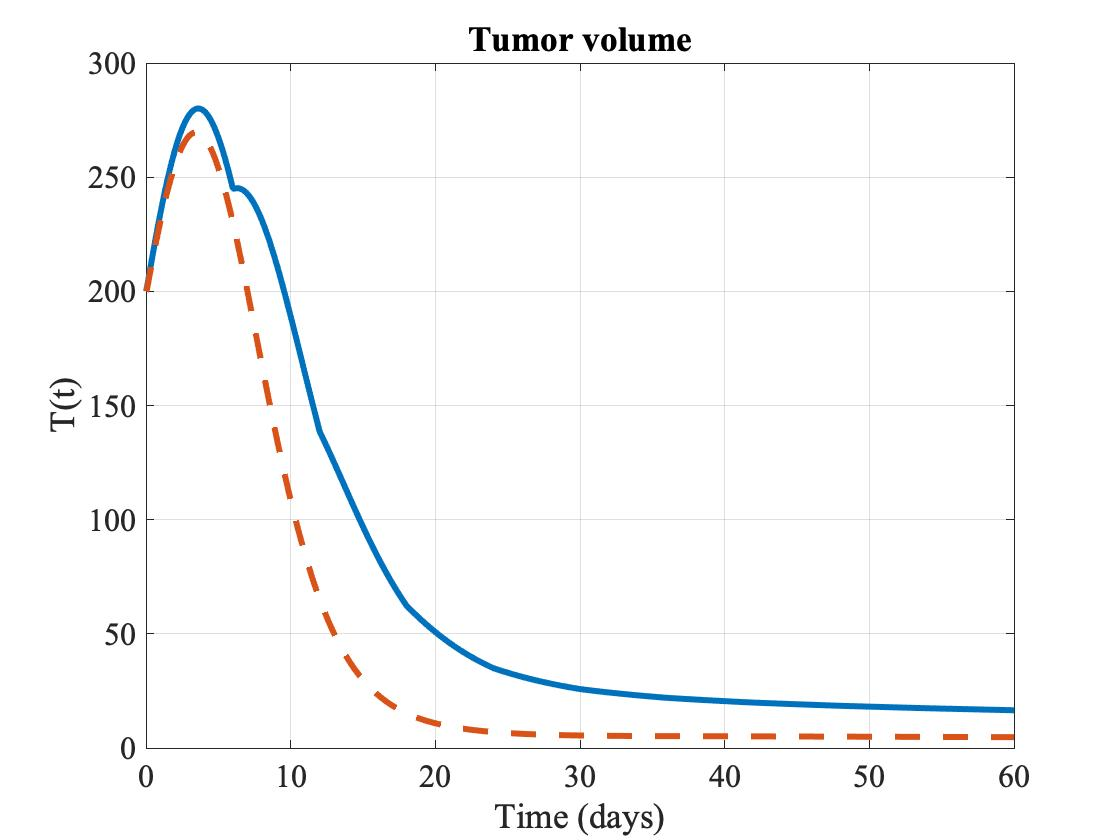
\includegraphics[width=0.49\textwidth]{fig/chemo_2.jpeg}
%		\caption{}
%	\end{subfigure}
%	\begin{subfigure}[b]{\textwidth}
%		\centering
%		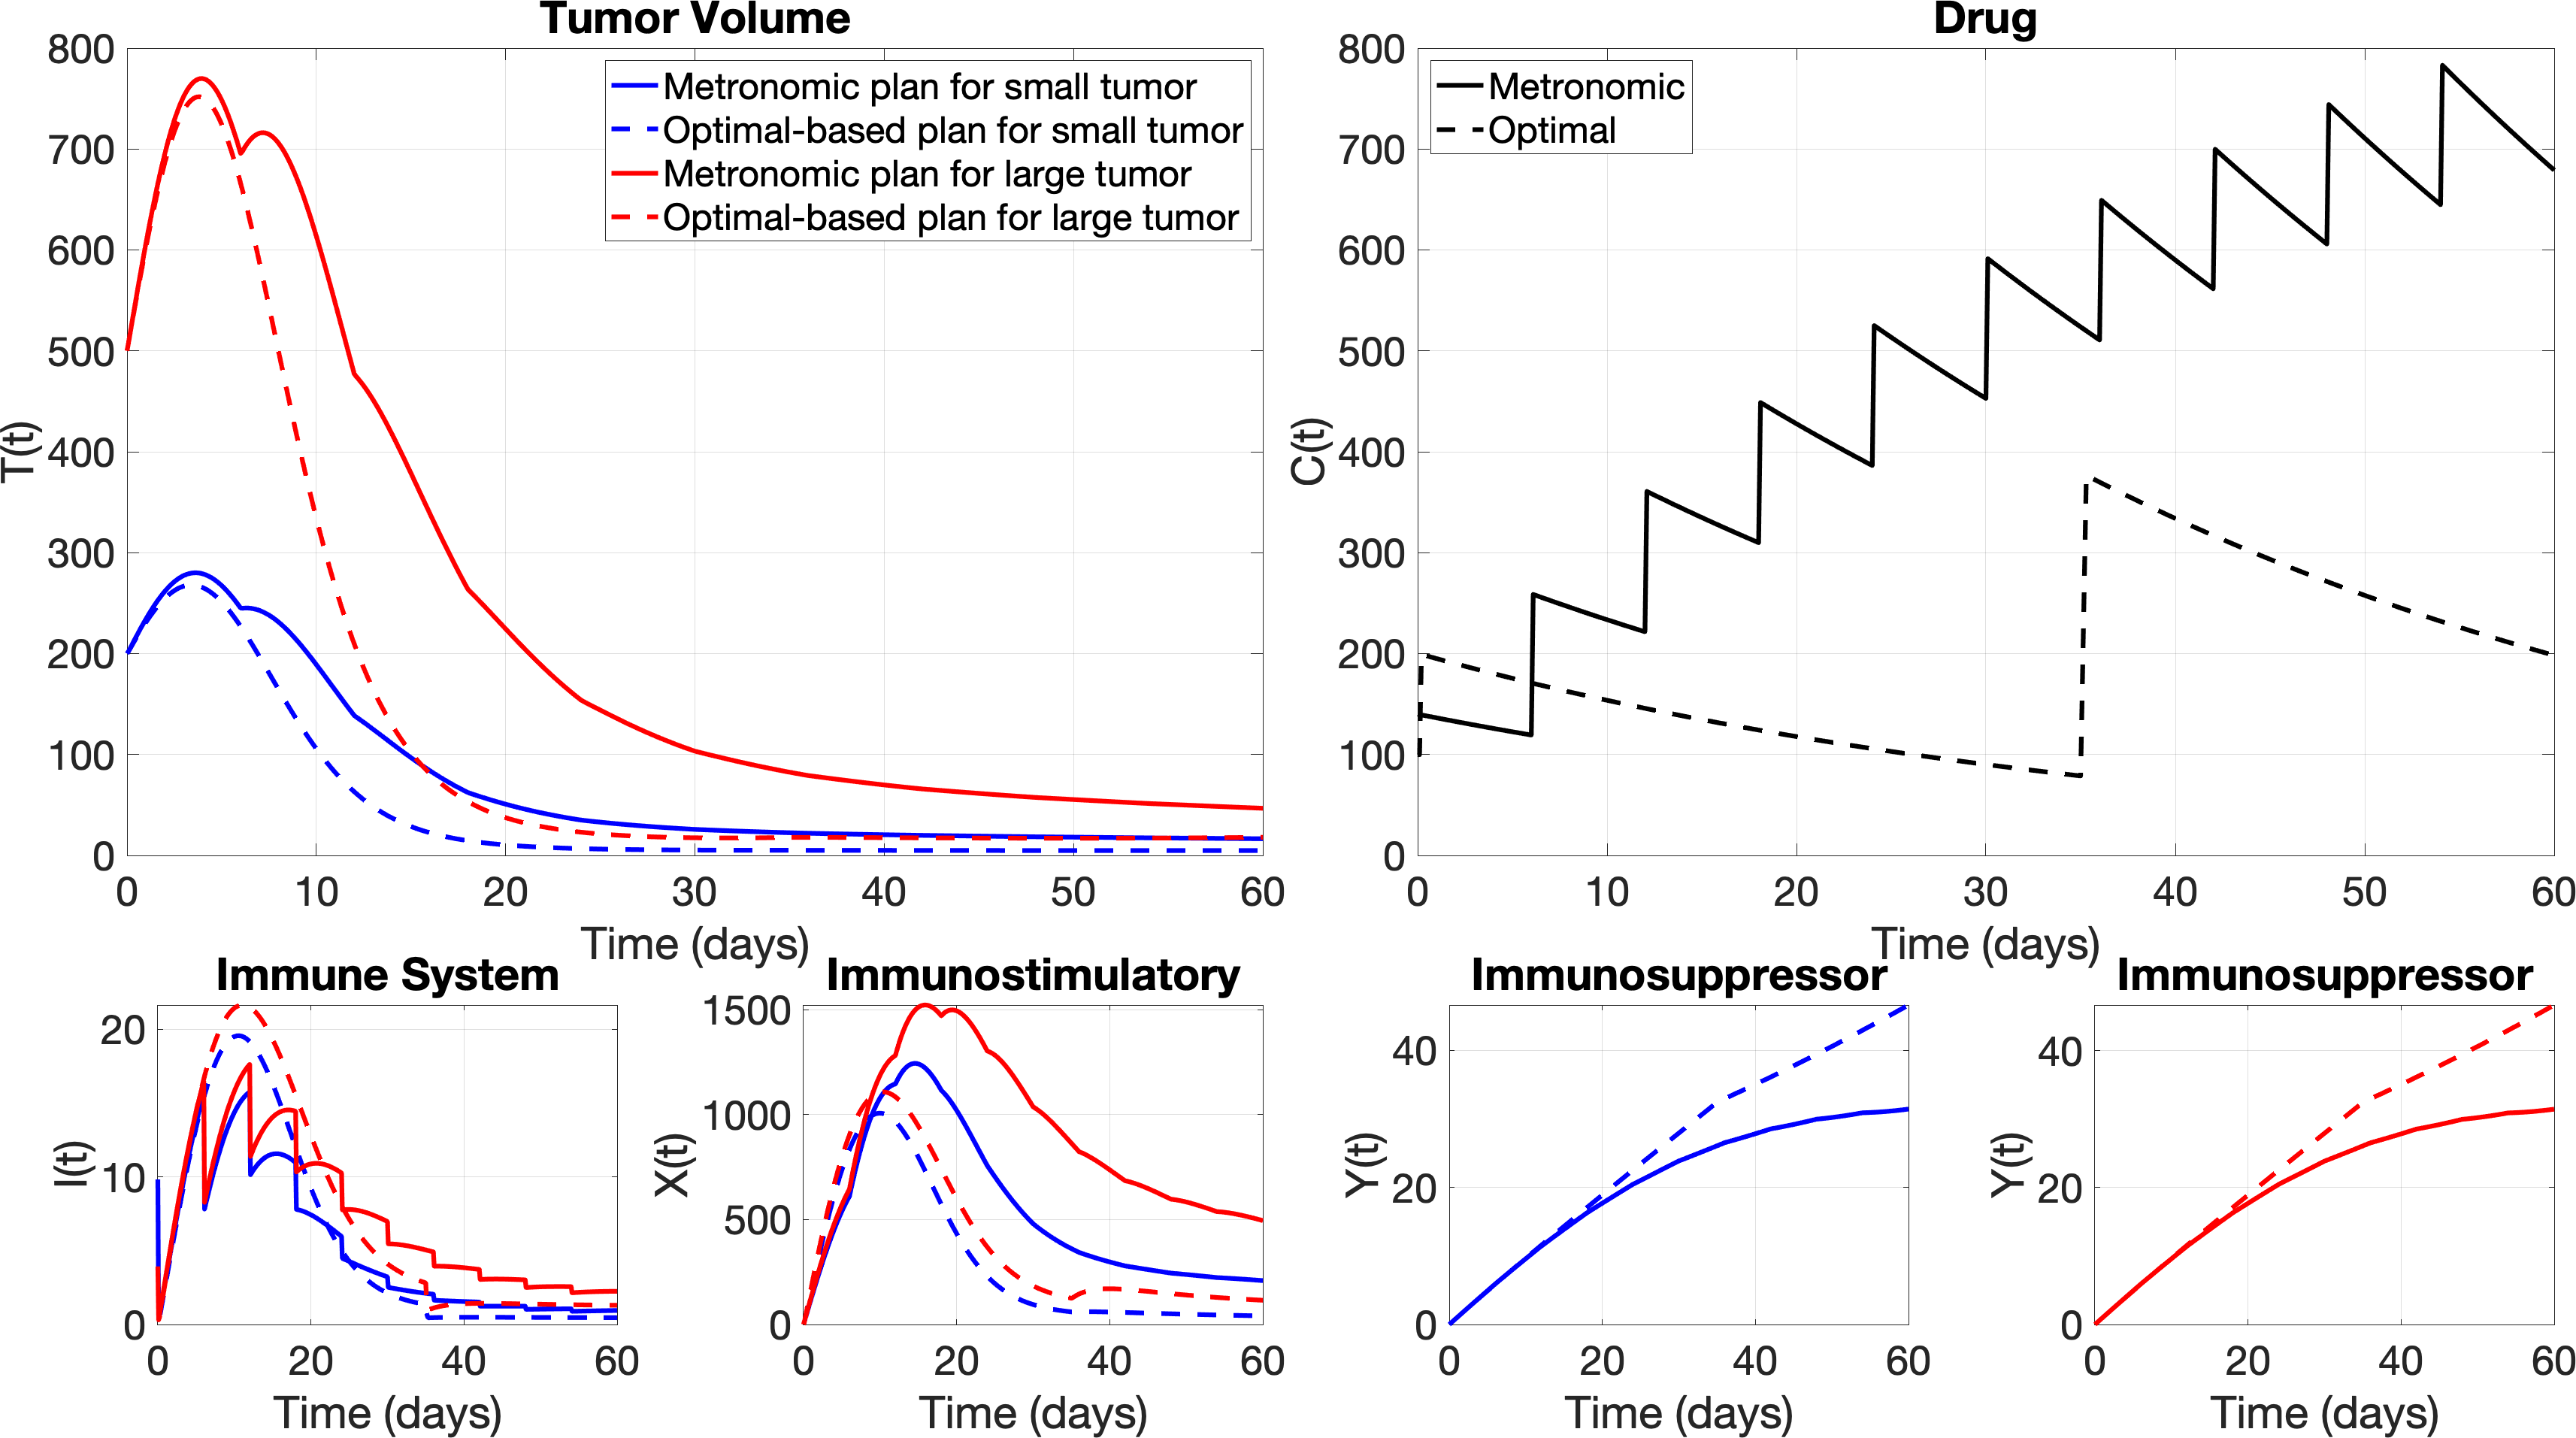
\includegraphics[width=1\textwidth]{fig/chemo_3.png}
%		\caption{}
%	\end{subfigure}
%	
%	\caption{Comparing a standard 140 mg/kg Q6D metronomic treatment with the obtained optimal control results. In (a), the tumor volume over the time for a metronomic chemotherapy with dose of 140mg/kg for every 6 days (solid line) compared with the final results of numerical optimal control (dashed line). In (b), a complete comparison between the time trajectories of the metronomic chemotherapy treatment plan with 140 mg/kg dose for every 6 days, and an \textit{optimal-based} treatment plan, that includes only two doses of chemotherapy (200 mg/kg at $t=0$ and 300 mg/kg at $t=35$), which is motivated by the numerical optimal control results. Tumor volume $T(t)$ is on the top left and drug kinetics term $C(t)$ is on the top right. Note that, our model assumes that the drug kinetics is independent of the tumor volume. Immune system, immunostimulatory and immunosuppresive are printed on the bottom with the same line type and colors.}
%	\label{fig:oc}
%\end{figure}
%
%\begin{figure}[H]
%	\centering
%	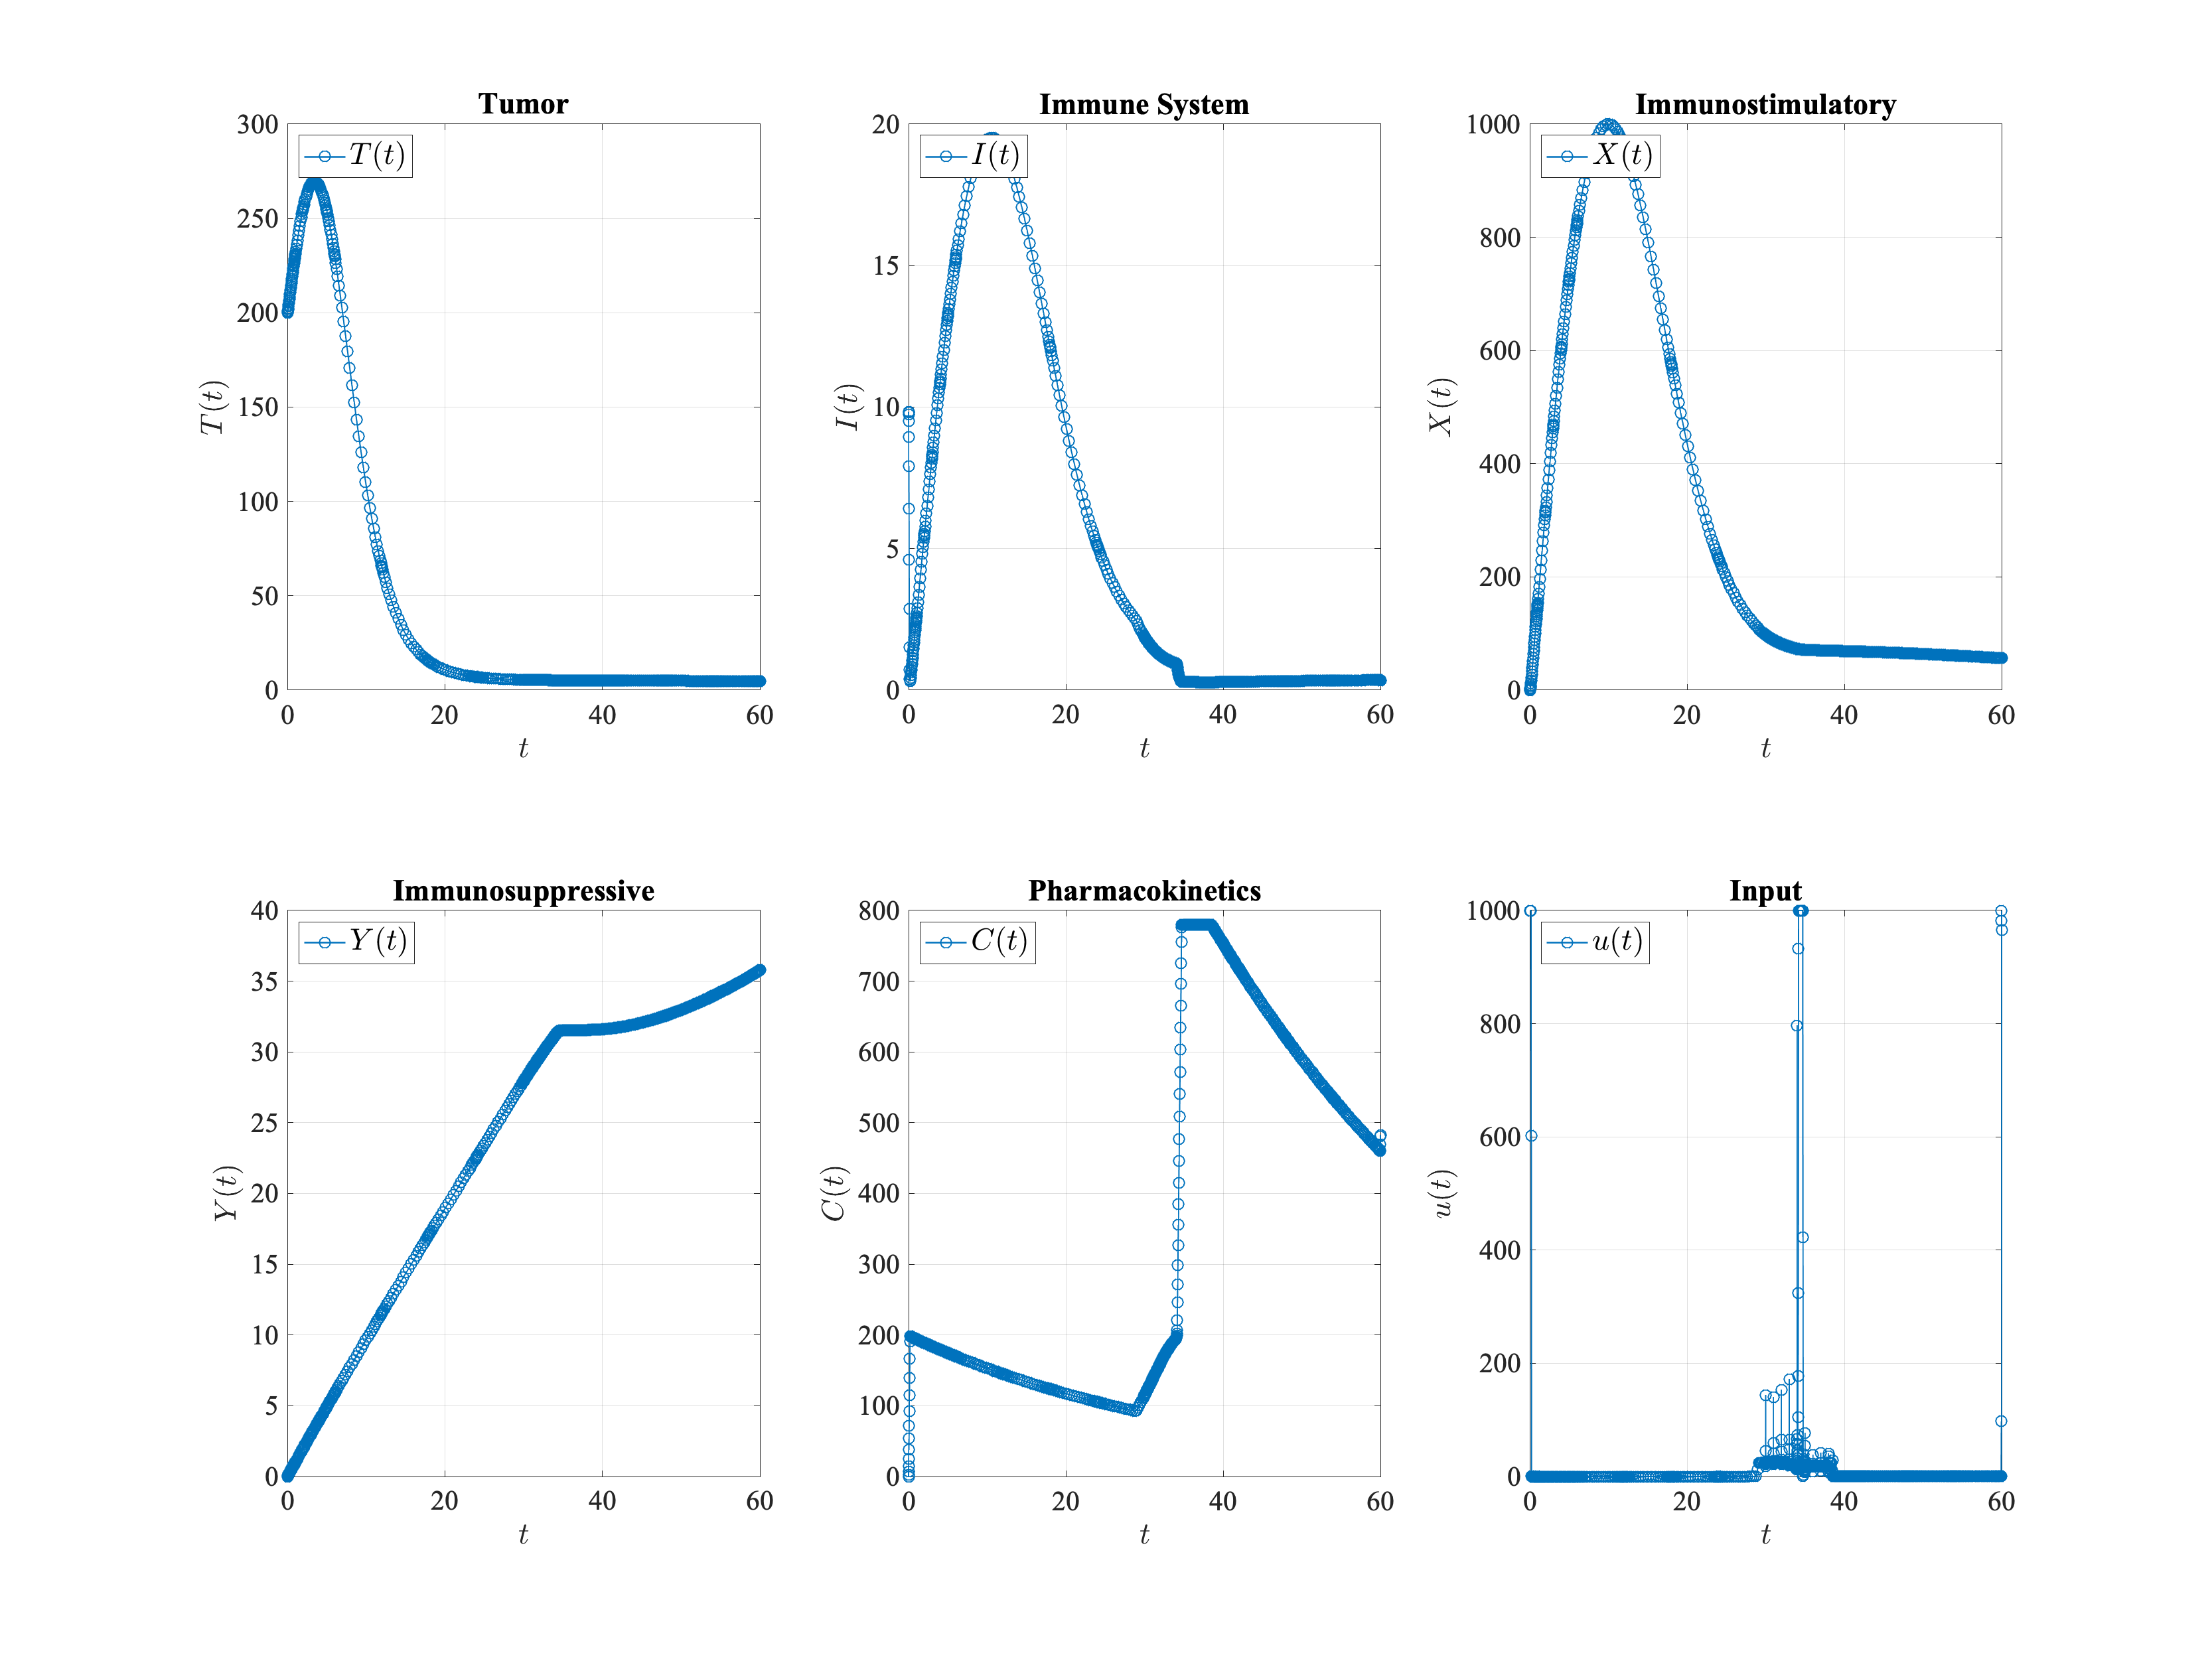
\includegraphics[width=1\textwidth]{fig/TumorSize_60_Final2Trajectories.png}
%	\caption{Time trajectories of the state variables of the optimally controlled input. Boundary conditions are $C_m=780$, $T_m=4000$, $I_m=100$, $X_m=1000$, $Y_m=1000$, $u_m=1000$, and $U_m=1400$. Circles show the final collocation points. A higher density of circles on a line represent more computational complexity of the numerical solver.}
%	\label{fig:OP1}
%\end{figure}
%
%\begin{figure}[H]
%	\centering
%	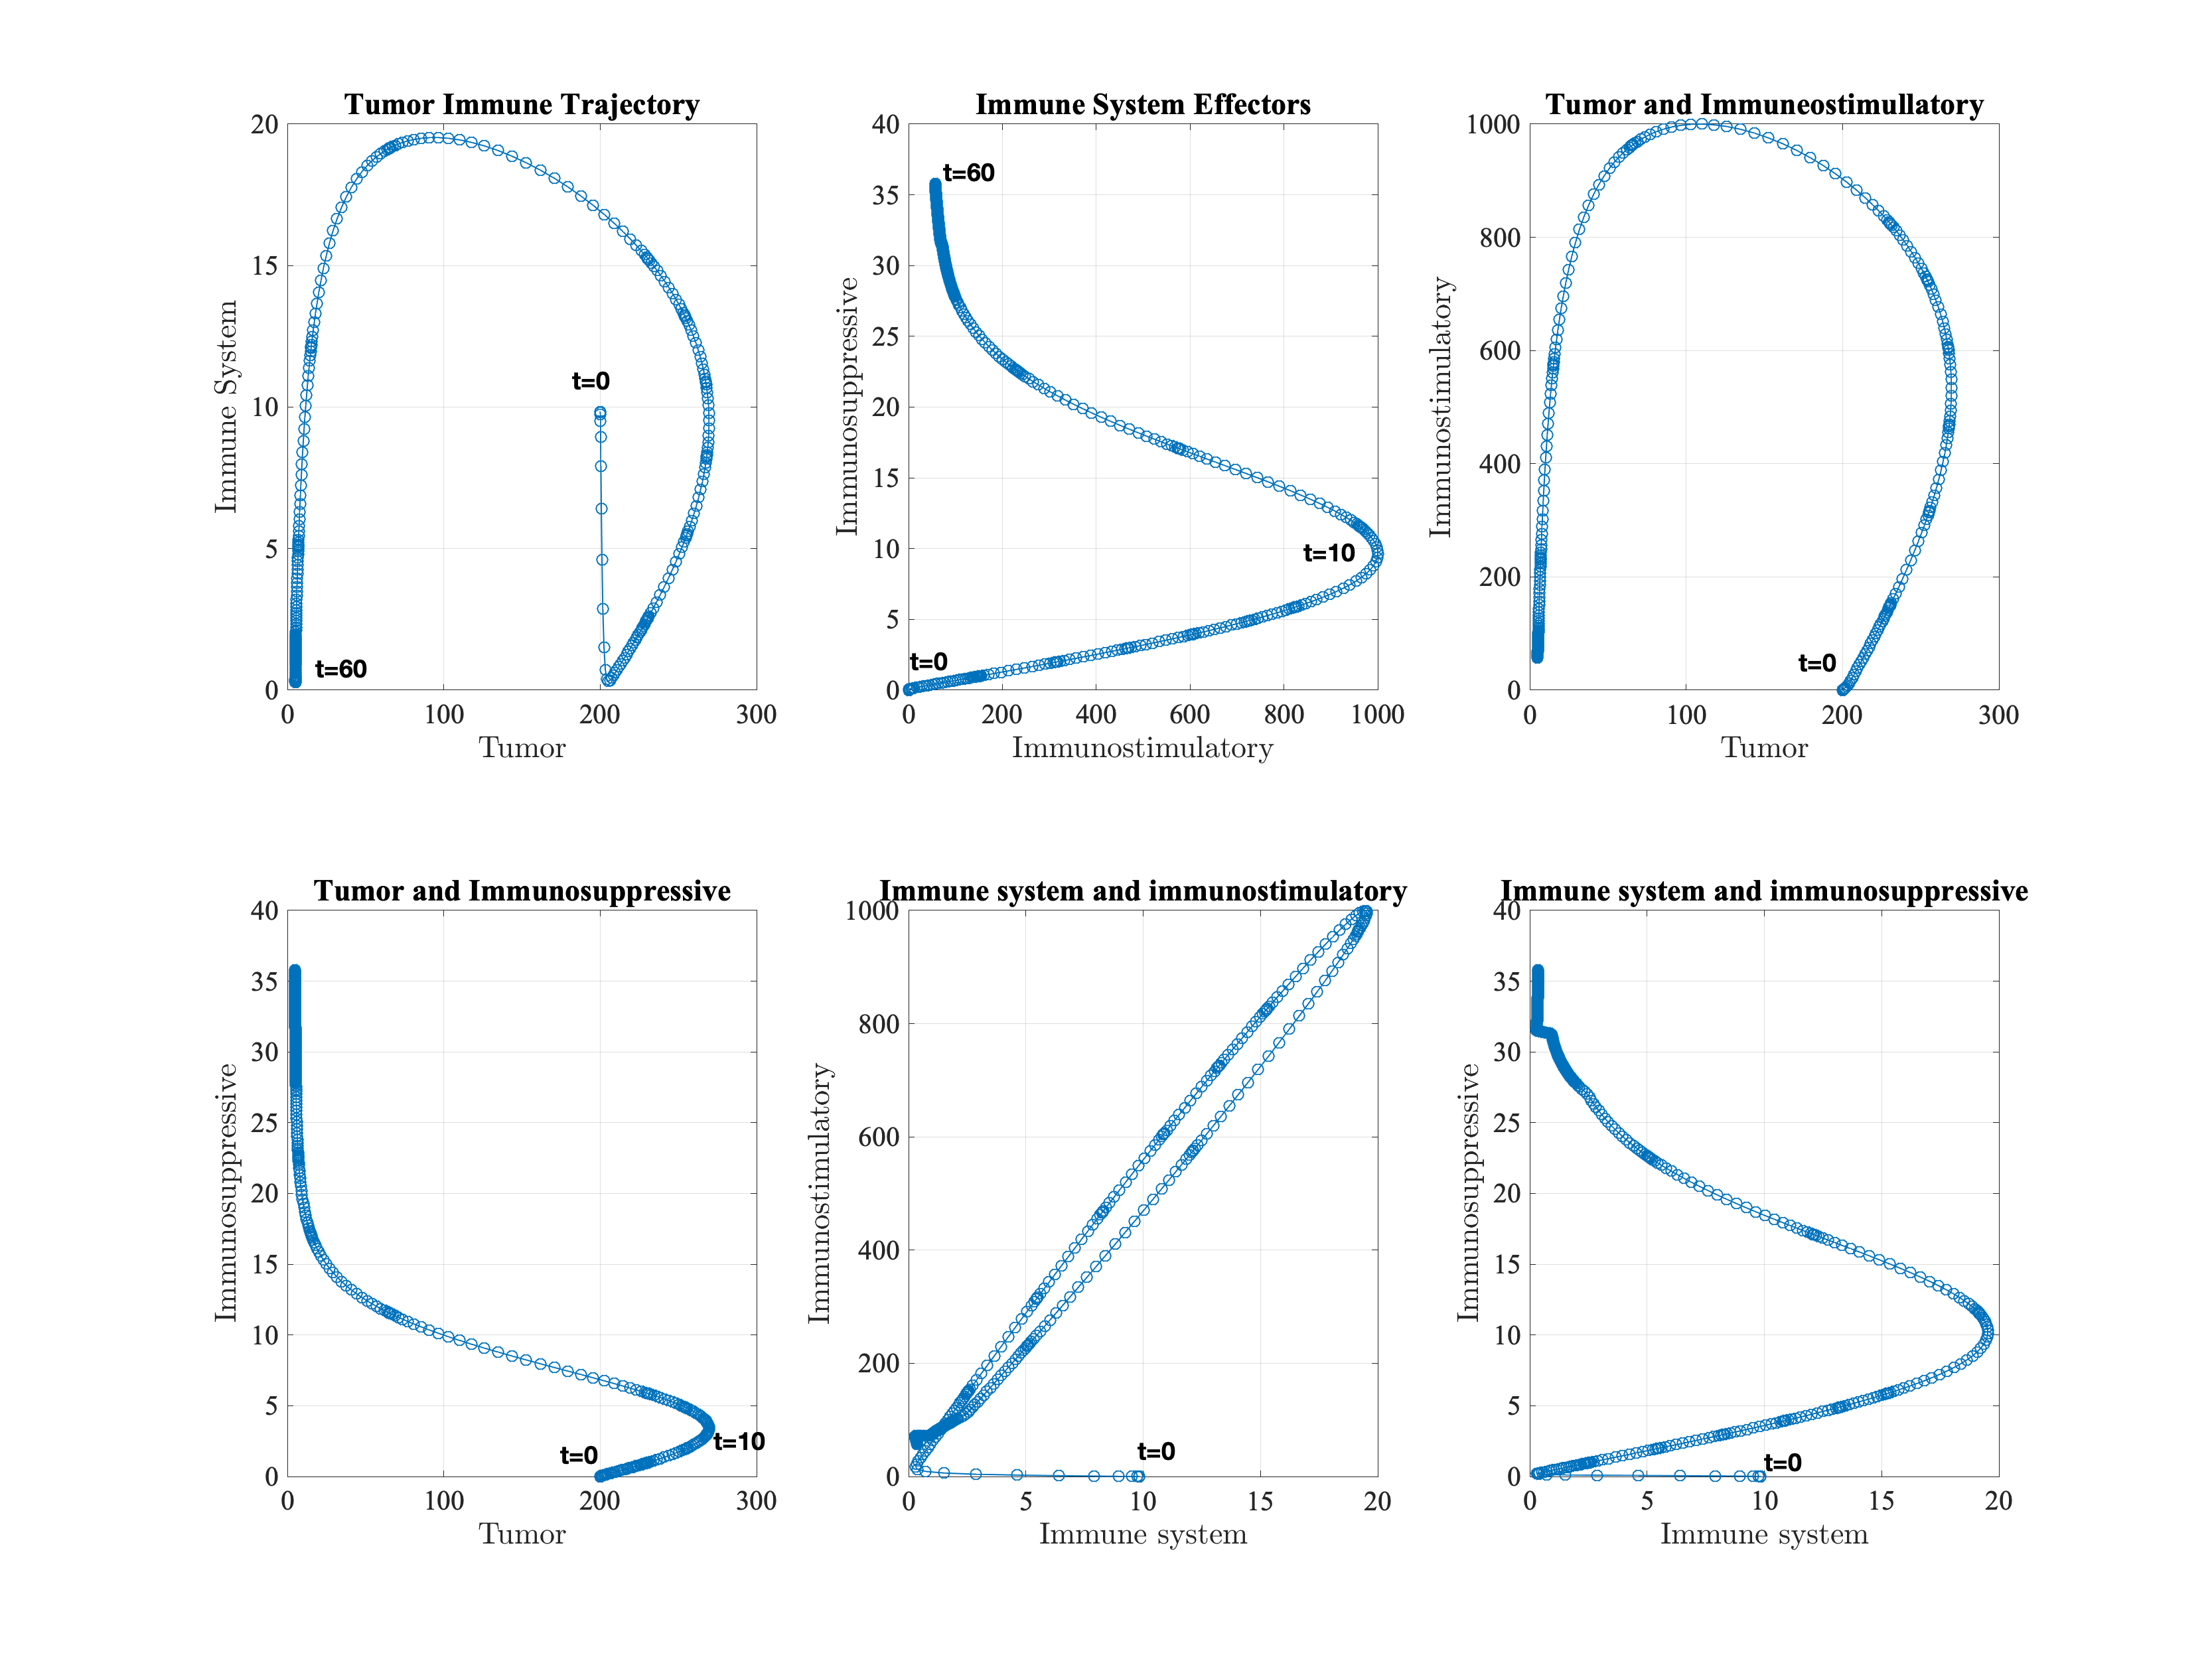
\includegraphics[width=1\textwidth]{fig/TumorSize_60_Final2Immune.png}
%	\caption{Projection of state variables presented in Figure~\ref{fig:OP1}. Circles show the final collocation points. A higher density of circles on a line represent more computational complexity of the numerical solver.}
%	\label{fig:OP2}
%\end{figure}
%
%\begin{figure}[H]
%	\centering
%	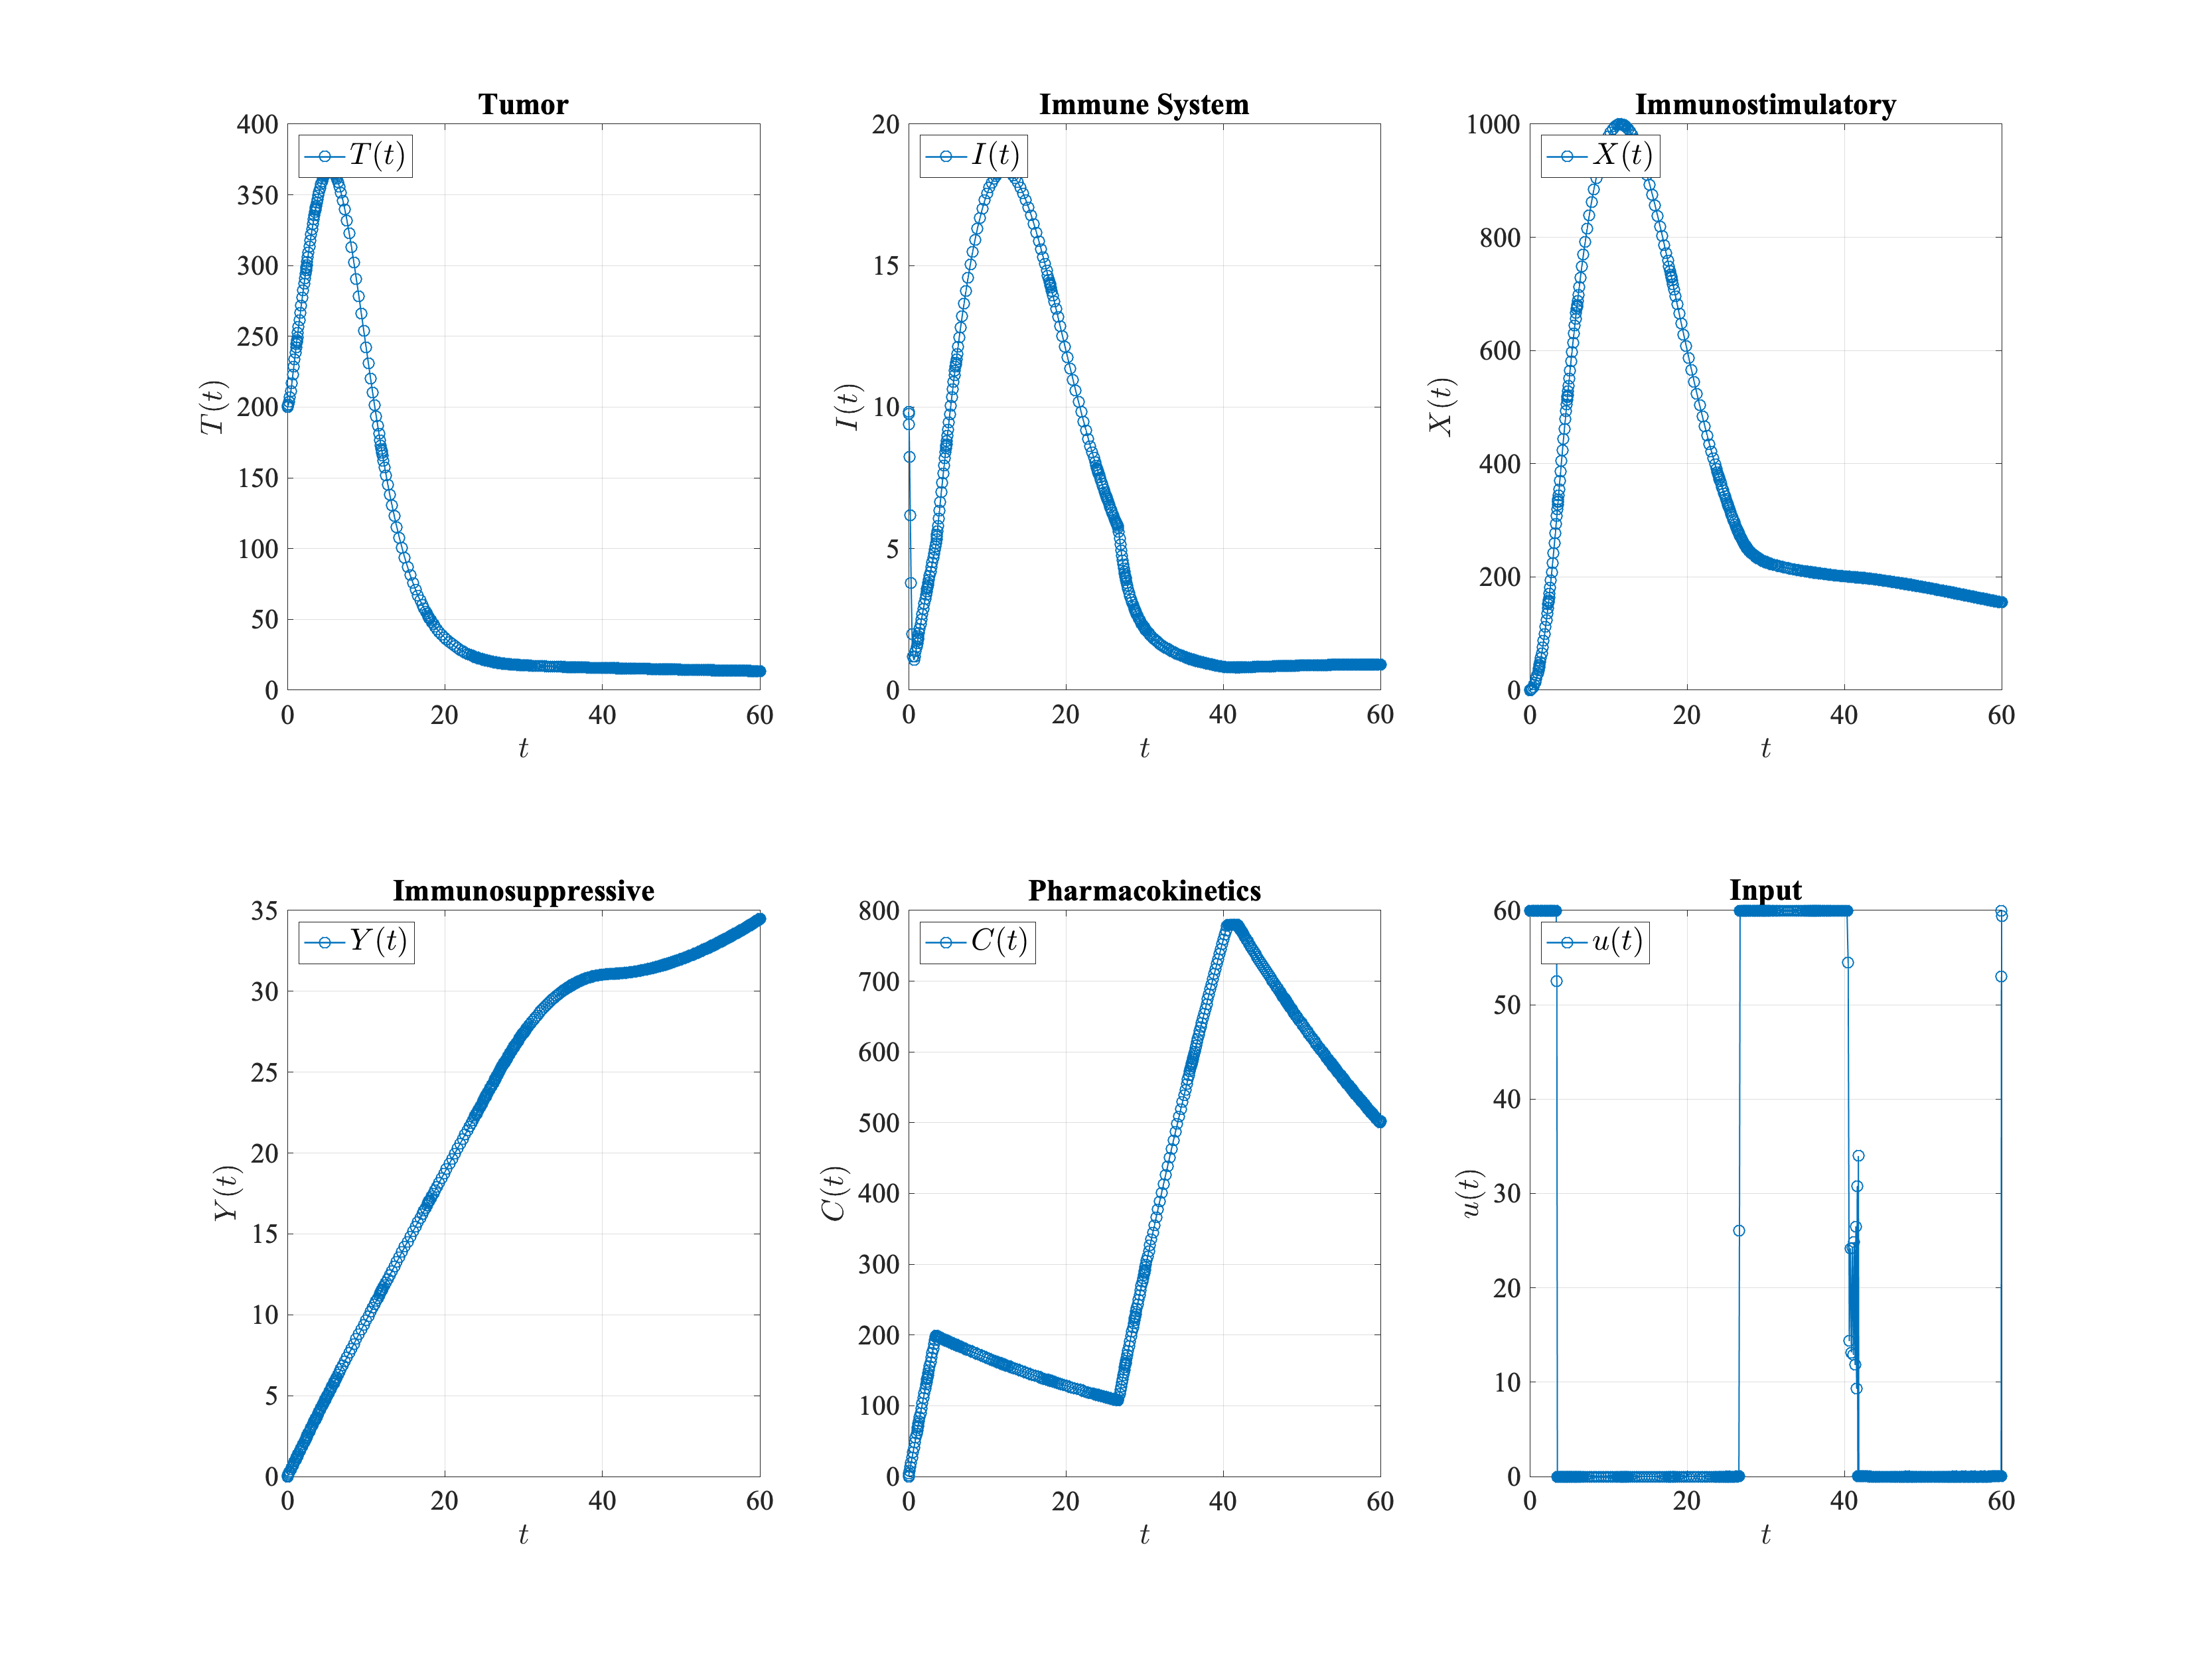
\includegraphics[width=1\textwidth]{fig/TumorSize_60_FinalTrajectories.png}
%	\caption{Time trajectories of the state variables of the optimally controlled input with a lower bound. Boundary conditions are $C_m=780$, $T_m=4000$, $I_m=100$, $X_m=1000$, $Y_m=1000$, $u_m=60$, and $U_m=1400$. Circles show the final collocation points. A higher density of circles on a line represent more computational complexity of the numerical solver.}
%	\label{fig:OP3}
%\end{figure}
%
%\begin{figure}[H]
%	\centering
%	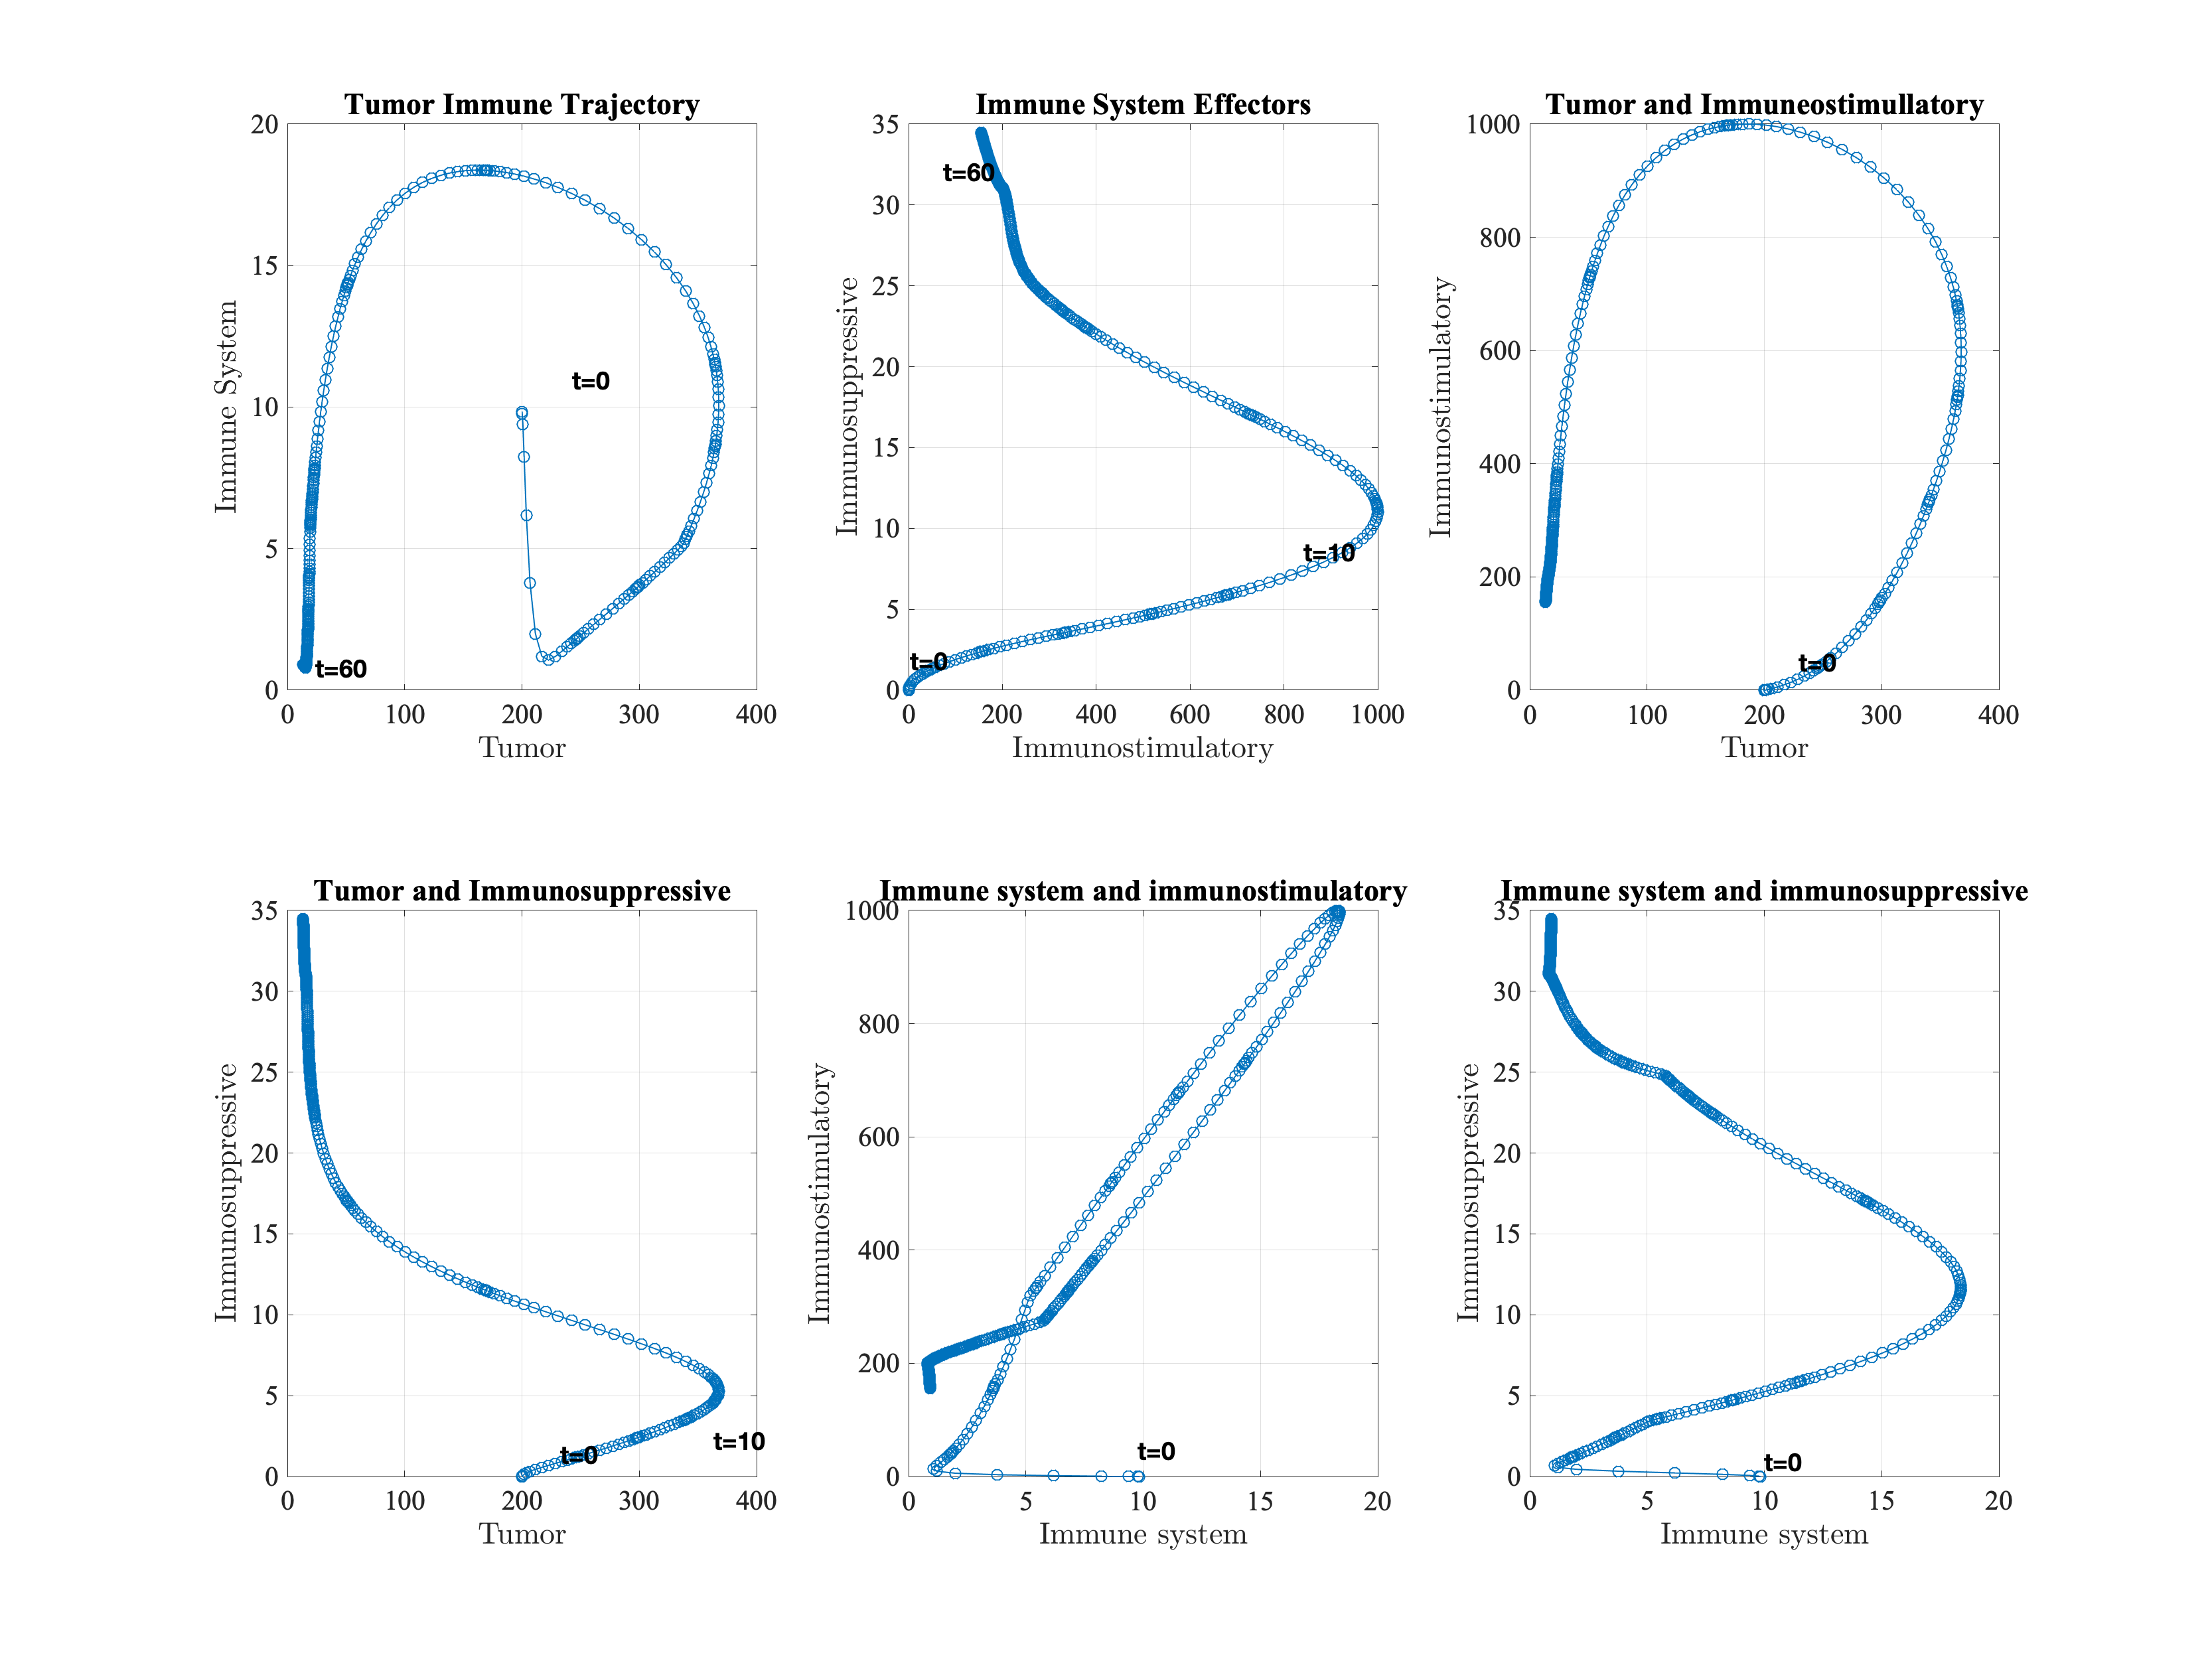
\includegraphics[width=1\textwidth]{fig/TumorSize_60_FinalImmune.png}
%	\caption{Projection of state variables presented in Figure~\ref{fig:OP3}. Circles show the final collocation points. A higher density of circles on a line represent more computational complexity of the numerical solver.}
%	\label{fig:OP4}
%\end{figure}
